% Capítulo 2. Marco teórico
% Estructura según índice de la Dra. Lárraga.

\chapter{Marco teórico}
\label{ch:marco-teorico}

\begin{resumen}
Este capítulo revisa la literatura relevante sobre crecimiento urbano, modelos espaciales y técnicas de modelado. Se presenta la motivación del estudio, la justificación de la integración AC+AG y el contexto mexicano y latinoamericano. Se describen los fundamentos de Weight of Evidence, Autómatas Celulares y Algoritmos Genéticos, así como las métricas de evaluación espacial (IoU, Kappa, FoM) utilizadas para validación. Se incluye la revisión de literatura y el posicionamiento del enfoque WoE-AC en el estado del arte.
\end{resumen}

\section{Crecimiento urbano}

El crecimiento urbano en México y en el mundo ejerce presión creciente sobre ecosistemas, infraestructura y calidad de vida. Esta expansión urbana acelerada presenta desafíos multidimensionales que requieren herramientas de modelado y predicción más sofisticadas.

\subsection{Presiones ambientales y sociales}

El crecimiento urbano descontrolado genera múltiples impactos interrelacionados. La degradación ambiental se manifiesta en pérdida de biodiversidad, contaminación y fragmentación de ecosistemas. Los sistemas de transporte, agua y energía experimentan sobrecarga ante demandas crecientes. Se profundiza la inequidad social mediante segregación espacial y acceso desigual a servicios urbanos. Adicionalmente, la conversión irreversible de tierras productivas reduce la capacidad de producción alimentaria regional.

\subsection{Limitaciones de los enfoques tradicionales}

Los métodos convencionales de planificación urbana presentan limitaciones estructurales. Predominan los enfoques reactivos que responden a cambios ya ocurridos en lugar de anticiparlos. Los modelos empleados resultan excesivamente simplificados para capturar la complejidad de las dinámicas urbanas reales. La falta de validación temporal implica que las predicciones rara vez se contrastan con datos históricos extensos. Finalmente, la dependencia excesiva de la experiencia e intuición del planificador introduce sesgos humanos que afectan la calidad de las decisiones.

\subsection{Motivación del estudio}

\subsubsection{Necesidad de herramientas predictivas avanzadas}

\paragraph{Demanda de automatización}

La calibración manual de modelos urbanos presenta múltiples problemas que justifican la búsqueda de alternativas automatizadas. El proceso resulta intensivo en tiempo, requiriendo semanas o meses de ajuste manual. La falta de reproducibilidad implica que diferentes modeladores obtienen resultados distintos ante los mismos datos. La subjetividad inherente hace que los resultados sean influenciados por sesgos y preferencias del usuario. La exploración limitada del espacio de parámetros impide identificar configuraciones óptimas que podrían mejorar significativamente el desempeño.

\paragraph{Oportunidades tecnológicas}

El desarrollo tecnológico actual ofrece oportunidades sin precedentes para superar estas limitaciones. Las series temporales de datos satelitales de décadas están disponibles gratuitamente a través de plataformas como Google Earth Engine. El poder computacional permite procesamiento paralelo y optimización masiva a costos accesibles. Los algoritmos evolutivos han alcanzado madurez con técnicas probadas en múltiples dominios. El ecosistema de software open-source proporciona infraestructura robusta para investigación reproducible.

\subsubsection{Justificación de la integración AC + AG}

\paragraph{Complementariedad de enfoques}

Los Autómatas Celulares y Algoritmos Genéticos se complementan de manera natural:

\begin{table}[h]
\centering
\caption{Complementariedad entre AC y AG}
\renewcommand{\arraystretch}{1.3}
\begin{tabular}{@{}lll@{}}
\toprule
\textbf{Aspecto} & \textbf{Autómatas Celulares} & \textbf{Algoritmos Genéticos} \\
\midrule
Función principal & Simulación espacial & Optimización de parámetros \\
Fortalezas & Modelado de emergencia & Búsqueda en espacios complejos \\
Limitaciones & Calibración manual & Requiere función objetivo \\
Integración & Proporciona simulación & Optimiza parámetros del AC \\
\bottomrule
\end{tabular}
\label{tab:ac_ag_complementarity}
\end{table}

\paragraph{Ventajas de la integración}

La combinación AC + AG ofrece múltiples beneficios que superan las capacidades de cada técnica por separado. La automatización completa elimina la intervención manual en calibración, mientras que la exploración exhaustiva evalúa miles de combinaciones de parámetros sistemáticamente. La optimización multi-objetivo permite balancear múltiples criterios simultáneamente. La reproducibilidad asegura resultados consistentes entre diferentes ejecuciones, y la evaluación sistemática con métricas espaciales proporciona validación robusta.

\subsubsection{Contexto mexicano y latinoamericano}

\paragraph{Características específicas}

Las ciudades mexicanas presentan particularidades que justifican el desarrollo de modelos específicos. Las tasas de urbanización superan el promedio mundial, generando crecimiento acelerado que desborda la capacidad de planificación tradicional. Los asentamientos irregulares representan una proporción significativa del desarrollo urbano, pero no son capturados adecuadamente por modelos tradicionales diseñados para contextos formales. La topografía accidentada y las restricciones naturales generan geografías complejas que condicionan los patrones de expansión. Finalmente, las limitaciones de datos disponibles, aunque menores que en países desarrollados, pueden superarse mediante técnicas de sensado remoto.

\paragraph{Oportunidad de transferencia tecnológica}

El desarrollo de herramientas open-source adaptadas al contexto mexicano ofrece oportunidades significativas de transferencia tecnológica. Facilita la adopción por parte de gobiernos locales con recursos limitados, reduce costos de licenciamiento de software especializado, promueve la capacitación técnica local, y genera metodologías replicables en otros países latinoamericanos con características urbanas similares.

\subsubsection{Relevancia científica}

\paragraph{Contribución metodológica}

Este estudio aporta avances metodológicos significativos en cuatro dimensiones: la extracción de conocimiento mediante Weight of Evidence para guiar la optimización; la calibración multi-métrica integrando IoU, FOM y Kappa en la función objetivo; la validación temporal extensa utilizando series de 37 años (1984-2020); y la reproducibilidad extremo a extremo desde datos satelitales hasta resultados finales.

\paragraph{Impacto en el campo}

La investigación contribuye al avance del campo mediante el cierre de brechas en calibración reproducible de AC, la integración novedosa de técnicas complementarias (WoE, AC, AG), el desarrollo de pipelines modulares y reutilizables, y la validación con casos reales de complejidad significativa que demuestran la aplicabilidad práctica del enfoque.

\subsubsection{Urgencia de la problemática}

\paragraph{Ventana de oportunidad}

Varios factores convergen para hacer este momento especialmente oportuno para el desarrollo de herramientas predictivas urbanas. La Agenda 2030 y sus metas de desarrollo sostenible requieren herramientas predictivas para monitoreo de progreso. El cambio climático genera necesidad urgente de planificación adaptativa ante escenarios de incertidumbre. La digitalización gubernamental impulsa adopción creciente de herramientas tecnológicas en gestión pública. Las políticas de datos abiertos facilitan el acceso a información antes restringida.

\paragraph{Costo de la inacción}

La falta de herramientas predictivas adecuadas conlleva costos crecientes que justifican la inversión en investigación. La infraestructura inadecuada para el crecimiento real genera congestión, deficiencias en servicios y costos de operación elevados. La pérdida irreversible de recursos naturales compromete la sostenibilidad de largo plazo. La inequidad urbana creciente erosiona la cohesión social. Los costos de remediación resultan exponencialmente mayores que los de prevención mediante planificación informada.

Por tanto, el desarrollo de modelos predictivos automatizados representa no solo una oportunidad científica, sino una necesidad social urgente.

\section{Modelos de cambio de uso de suelo}

La aplicación de Deep Learning al análisis de imágenes satelitales ha abierto nuevas posibilidades para la detección automática de cambios urbanos. \textcite{Ma2019} aplicaron redes neuronales convolucionales para detección de cambios urbanos con alta precisión, mientras que \textcite{Gomez2020} desarrollaron un marco de modelado espaciotemporal de crecimiento urbano basado en aprendizaje automático.

Sin embargo, los enfoques de DL presentan limitaciones importantes: requieren grandes cantidades de datos etiquetados para entrenamiento, implican alto costo computacional en hardware especializado, y ofrecen menor interpretabilidad que los AC tradicionales, dificultando la explicación de las predicciones a tomadores de decisiones.

\section{Modelos espaciales de crecimiento urbano}

El modelado del crecimiento urbano mediante técnicas computacionales ha evolucionado significativamente en las últimas décadas, consolidándose como un área de investigación multidisciplinaria que combina geografía, ciencias de la computación, planificación urbana y ciencias ambientales.

\subsection{Fuentes de datos satelitales}

El desarrollo de plataformas satelitales como Landsat y Sentinel ha revolucionado el acceso a datos multitemporales de alta calidad. Los trabajos de \textcite{Herold2003} y \textcite{Gong2013} establecieron metodologías estándar para el procesamiento de series temporales satelitales.

\subsection{Revisión de literatura}

La literatura relevante revisada revela la siguiente distribución temática:

\begin{figure}[h]
\centering
\begin{tikzpicture}[scale=0.9]
\pie[
	sum=auto,
	after number=\ refs,
	radius=2.5,
	text=legend,
	color={blue!70,red!70,green!60,orange!70,purple!50},
	/tikz/every text node part/.style={align=left}
]{
	10/AC y SLEUTH,
	6/Calibración (GA-PSO-MOO),
	8/Sensado remoto y DL,
	4/Planeación e impacto,
	3/Herramientas open-source
}
\end{tikzpicture}
\caption{Distribución temática de la literatura revisada}
\label{fig:literature_distribution}
\end{figure}

De la literatura revisada, pocas referencias tratan directamente con la integración AC + AG, evidenciando una oportunidad de investigación:

\begin{figure}[h]
\centering
\begin{tikzpicture}
\begin{axis}[
	ybar,
	bar width=40pt,
	ymin=0,
	ymax=30,
	width=0.7\textwidth,
	height=0.4\textheight,
	symbolic x coords={AC+AG,Otros temas},
	xtick=data,
	nodes near coords,
	nodes near coords align={vertical},
	ylabel={Número de referencias},
	ymajorgrids=true,
	grid style=dashed,
	xlabel style={font=\large},
	ylabel style={font=\large}
]
	\addplot[fill=blue!70] coordinates {(AC+AG,6) (Otros temas,25)};
\end{axis}
\end{tikzpicture}
\caption{Distribución de enfoques AC+AG vs otros temas}
\label{fig:ac_ga_distribution}
\end{figure}

La revisión de literatura revela un balance entre fortalezas consolidadas y limitaciones persistentes. Entre las \textit{fortalezas identificadas}, los modelos AC y SLEUTH han demostrado robustez en múltiples regiones del mundo; la optimización evolutiva mejora consistentemente la concordancia con datos observados; el sensado remoto proporciona insumos multitemporales de alta calidad; y el ecosistema open-source habilita la reproducibilidad científica.

Las \textit{limitaciones identificadas} incluyen la calibración manual intensiva en enfoques tradicionales, el costo computacional elevado en métodos evolutivos, la dependencia de grandes datasets etiquetados en enfoques de DL, y la limitada integración entre diferentes técnicas complementarias.

Se identifican cuatro \textit{brechas de investigación} principales que motivan el presente trabajo: la necesidad de métodos de calibración reproducibles y no sesgados; la integración efectiva multi-técnica combinando AC, AG y análisis espacial; la validación temporal robusta utilizando series temporales extensas; y la adaptación de metodologías a contextos mexicanos y latinoamericanos, donde las dinámicas de crecimiento urbano difieren de los contextos donde se han desarrollado la mayoría de las herramientas existentes.

\section{Autómatas celulares aplicados al crecimiento urbano}

\subsection{Autómatas Celulares en modelado urbano}

Los Autómatas Celulares (AC) han demostrado ser una herramienta fundamental para el modelado de sistemas complejos espaciales. Los trabajos pioneros de \textcite{Wolfram1984} establecieron las bases teóricas, mientras que \textcite{Clarke1998} y \textcite{White1997} fueron los primeros en aplicar AC específicamente al crecimiento urbano.

Los AC son efectivos para capturar dinámicas espaciales a partir de reglas locales, permitiendo que patrones complejos emerjan de interacciones simples entre celdas vecinas. Esta característica los hace particularmente adecuados para modelar fenómenos urbanos, donde las decisiones locales de uso de suelo pueden generar patrones metropolitanos complejos.

\subsection{El modelo SLEUTH}

El modelo SLEUTH (Slope, Land use, Exclusion, Urban extent, Transportation, Hillshade), desarrollado por \textcite{Clarke2007}, representa uno de los enfoques más consolidados en el modelado AC urbano. SLEUTH ha sido probado en múltiples regiones del mundo, demostrando su robustez y capacidad de generalización.

Sin embargo, SLEUTH presenta limitaciones significativas. La calibración manual intensiva requiere ajuste de múltiples parámetros por parte de un operador experimentado, generando dependencia del modelador y resultados que pueden variar según la experiencia del usuario. El proceso es laborioso, con limitada automatización, y propenso a sesgos humanos que afectan la reproducibilidad de los estudios.

\section{Método Weight of Evidence (WoE)}

El ecosistema de código abierto ha habilitado la reproducibilidad y transferencia tecnológica en modelado urbano. DEAP \parencite{Fortin2024} proporciona un framework flexible para implementación de algoritmos evolutivos, mientras que Repast \parencite{North2023} ofrece una plataforma robusta de simulación basada en agentes. Para modelado urbano integrado, UrbanSim \parencite{Waddell2002} combina simulación de transporte y uso de suelo, y PyLUSAT \parencite{Chen2022} provee herramientas Python específicas para análisis de cambio de uso de suelo.

\section{Integración de Weight of Evidence y Autómatas Celulares}

\subsection{Algoritmos Genéticos para calibración}

La integración de Algoritmos Genéticos (AG) con AC urbanos representa una línea de investigación en crecimiento que aborda las limitaciones de calibración manual, con trabajos pioneros que demostraron la viabilidad del enfoque.

Estudios posteriores han expandido este enfoque mediante calibración automática con múltiples objetivos e integración de restricciones espaciales. Más recientemente, \textcite{Wang2021} acoplaron AC y AG para optimizar la forma urbana y la vitalidad en Wuhan, y \textcite{Tang2024} propusieron el modelo GSA-CA con algoritmos heurísticos para simular crecimiento urbano en regiones áridas.

\subsection{Otras técnicas de optimización}

Además de los AG, se han explorado otras metaheurísticas para la calibración de modelos urbanos. Particle Swarm Optimization (PSO) se ha aplicado para optimización continua de parámetros, mientras que técnicas de Multi-Objective Optimization (MOO) permiten balancear múltiples criterios de planificación simultáneamente. También se han desarrollado algoritmos híbridos que combinan las fortalezas de diferentes enfoques evolutivos.

\subsection{Impacto esperado}

El desarrollo de un modelo evolutivo AC+AG para simular y predecir el crecimiento urbano tiene el potencial de generar impacto significativo en múltiples dimensiones: científica, social y tecnológica.

\subsubsection{Impacto científico}

\paragraph{Avances metodológicos}

Esta investigación contribuye al avance del conocimiento científico mediante el cierre de brechas metodológicas reconocidas en la literatura, particularmente la problemática de calibración reproducible en Autómatas Celulares urbanos. La integración innovadora combina Weight of Evidence (WoE), Algoritmos Genéticos y métricas espaciales en un framework coherente. La validación robusta utiliza series temporales de 37 años, superando significativamente los estándares típicos de 2-3 puntos temporales. Los pipelines completamente automatizados aseguran reproducibilidad extremo a extremo desde datos crudos hasta resultados finales.

\paragraph{Contribuciones al campo}

Las contribuciones específicas incluyen la primera implementación completa de una metodología híbrida que integra extracción automática de conocimiento espacial con optimización evolutiva para calibración de AC urbanos. Se desarrolla un framework multi-métrico con función objetivo que balancea IoU, FOM y Kappa para evaluación integral. Se establece un protocolo de validación temporal como metodología estándar para modelos predictivos urbanos con series históricas extensas. La arquitectura modular facilita la extensión y adaptación a diferentes contextos urbanos.

\paragraph{Potencial de publicación}

Los resultados esperados tienen potencial para generar publicaciones de alto impacto en revistas especializadas como \emph{Computers, Environment and Urban Systems} y \emph{Urban Studies} en modelado urbano; \emph{Applied Soft Computing} y \emph{Evolutionary Computation} en métodos computacionales; \emph{Remote Sensing of Environment} e \emph{ISPRS Journal} en sensado remoto; así como en conferencias especializadas como AAIA, GECCO, IGARSS y Urban Remote Sensing Event.

\subsubsection{Impacto social}

\paragraph{Beneficios para la planificación urbana}

El modelo desarrollado proporcionará herramientas directamente aplicables para planificación proactiva mediante identificación temprana de áreas de probable expansión urbana. Facilitará la conservación dirigida al identificar áreas naturales en riesgo de urbanización para protección prioritaria. Permitirá evaluación de políticas mediante simulación de impactos de diferentes opciones de desarrollo antes de su implementación. Contribuirá a la transparencia gubernamental al proporcionar herramientas objetivas y reproducibles para justificación de decisiones.

\paragraph{Beneficios para tomadores de decisiones}

Los tomadores de decisiones se beneficiarán de la reducción de sesgos mediante decisiones basadas en evidencia cuantitativa. Contarán con capacidad de evaluación de escenarios para simular múltiples futuros alternativos. El modelo incorpora sistemáticamente sensibilidad a restricciones ambientales, topográficas y regulatorias. Las visualizaciones claras facilitarán la comunicación efectiva con ciudadanos y medios.

\paragraph{Contribución al desarrollo sostenible}

El proyecto contribuye directamente a varios Objetivos de Desarrollo Sostenible:

\begin{table}[h]
\centering
\caption{Contribución a los ODS}
\renewcommand{\arraystretch}{1.3}
\begin{tabular}{@{}clp{8cm}@{}}
\toprule
\textbf{ODS} & \textbf{Objetivo} & \textbf{Contribución del proyecto} \\
\midrule
11 & Ciudades sostenibles & Herramientas para planificación urbana inclusiva y sostenible \\
13 & Acción climática & Modelos para adaptación urbana al cambio climático \\
15 & Vida terrestre & Identificación de áreas naturales prioritarias para conservación \\
16 & Instituciones sólidas & Transparencia y evidencia en toma de decisiones públicas \\
\bottomrule
\end{tabular}
\label{tab:ods_contribution}
\end{table}

\subsubsection{Impacto tecnológico}

\paragraph{Desarrollo de capacidades técnicas}

El proyecto impulsa el desarrollo de capacidades técnicas locales mediante la adopción estratégica de tecnologías open-source como DEAP, Repast, UrbanSim y PyLUSAT. El diseño para escalabilidad computacional permite procesamiento distribuido en GPU y clusters, aprovechando infraestructura computacional moderna. La compatibilidad nativa con sistemas de información geográfica estándar facilita la integración con SIG existentes. Las interfaces accesibles permiten uso por planificadores sin formación técnica especializada.

\paragraph{Transferencia tecnológica}

El proyecto facilitará la transferencia tecnológica mediante liberación completa del código fuente bajo licencias permisivas, documentación completa con manuales técnicos y de usuario, ejemplos de casos de estudio en contextos mexicanos, y desarrollo de materiales educativos para capacitación de funcionarios públicos.

\paragraph{Innovación en el ecosistema}

La contribución al ecosistema tecnológico incluye establecimiento de estándares metodológicos para modelado urbano evolutivo, desarrollo de interfaces estándar para interoperabilidad con otras herramientas, arquitectura modular extensible para adición de nuevos métodos y fuentes de datos, y fomento de una comunidad de práctica de usuarios y desarrolladores en América Latina.

\subsubsection{Impacto específico en México}

\paragraph{Fortalecimiento institucional}

El proyecto contribuye al fortalecimiento institucional en múltiples niveles. CONAPO se beneficiará de herramientas para proyecciones urbanas más precisas. SEDATU contará con instrumentos para la política nacional de desarrollo urbano. Los gobiernos locales desarrollarán capacidades técnicas para planificación metropolitana. Las universidades fortalecerán sus programas de posgrado en estudios urbanos con casos de aplicación relevantes.

\paragraph{Ventajas competitivas}

El desarrollo de capacidades locales en modelado urbano avanzado reducirá la dependencia de consultorías internacionales costosas, generará metodologías adaptadas a contextos mexicanos específicos, creará oportunidades de exportación de servicios técnicos a otros países latinoamericanos, y posicionará a México como líder regional en innovación urbana.

\subsubsection{Impacto a largo plazo}

\paragraph{Transformación del campo}

Se espera que este trabajo contribuya a la democratización del modelado urbano mediante herramientas accesibles para instituciones con recursos limitados, la estandarización metodológica con protocolos reproducibles, la integración interdisciplinaria como puente entre ciencias de la computación, geografía y planificación, y la formación de recursos humanos con capacidades únicas en la intersección de múltiples disciplinas.

\paragraph{Escalabilidad del impacto}

La metodología desarrollada tiene potencial de aplicación en:

\begin{itemize}
	\item \textbf{Escala nacional}: Adaptación a las 384 áreas urbanas de México
	\item \textbf{Escala regional}: Transferencia a países con características similares
	\item \textbf{Escala global}: Contribución a iniciativas internacionales de monitoreo urbano
	\item \textbf{Escala temporal}: Aplicación a estudios de cambio climático y escenarios futuros
\end{itemize}

El impacto multidimensional esperado justifica la inversión en esta investigación como una contribución significativa tanto al avance del conocimiento científico como al bienestar social y al desarrollo tecnológico nacional.

\section{Evaluación de modelos predictivos}

\subsection{Matriz de confusión}

\subsubsection{Fundamento Teórico}

Sea $\Omega \subset \mathbb{R}^2$ el dominio espacial de estudio discretizado en $N = |\Omega|$ píxeles. Para cada píxel $i \in \Omega$, sea $y_i \in \{0, 1\}$ el estado observado real (donde 0 denota no-urbano y 1 denota urbano), y sea $\hat{y}_i \in \{0, 1\}$ el estado predicho por el modelo.

La \textbf{matriz de confusión} $\mathbf{C} \in \mathbb{N}^{2 \times 2}$ cuantifica la concordancia píxel a píxel entre predicción y observación mediante la estructura:

\begin{equation}
\mathbf{C} = \begin{pmatrix}
TN & FP \\
FN & TP
\end{pmatrix}
\label{eq:confusion_matrix}
\end{equation}

donde cada elemento se define formalmente como sigue. Sea $\mathbb{1}[\cdot]$ la función indicadora que toma valor 1 cuando su argumento es verdadero y 0 en caso contrario. Entonces, los \textbf{verdaderos positivos} se definen como

\begin{equation}
TP = \sum_{i \in \Omega} \mathbb{1}[\hat{y}_i = 1 \land y_i = 1]
\label{eq:tp}
\end{equation}

representando píxeles correctamente identificados como urbanos. Los \textbf{verdaderos negativos} se definen como

\begin{equation}
TN = \sum_{i \in \Omega} \mathbb{1}[\hat{y}_i = 0 \land y_i = 0]
\label{eq:tn}
\end{equation}

representando píxeles correctamente identificados como no-urbanos. Los \textbf{falsos positivos} se definen como

\begin{equation}
FP = \sum_{i \in \Omega} \mathbb{1}[\hat{y}_i = 1 \land y_i = 0]
\label{eq:fp}
\end{equation}

correspondiendo a errores de comisión (sobre-predicción de urbanización). Finalmente, los \textbf{falsos negativos} se definen como

\begin{equation}
FN = \sum_{i \in \Omega} \mathbb{1}[\hat{y}_i = 0 \land y_i = 1]
\label{eq:fn}
\end{equation}

correspondiendo a errores de omisión (sub-predicción de urbanización). Estos cuatro componentes satisfacen la propiedad de partición exhaustiva del dominio: $TP + TN + FP + FN = N$.

\subsubsection{Implementación}

La construcción de la matriz requiere correspondencia espacial exacta entre mapas predicho y observado, implicando idéntica resolución espacial, sistema de proyección cartográfica y extensión geográfica. Los píxeles se clasifican iterando sobre $\Omega$ y evaluando las condiciones lógicas de las ecuaciones \eqref{eq:tp}--\eqref{eq:fn}.

La magnitud relativa de $FP$ versus $FN$ revela sesgo sistemático del modelo: si $FP > FN$, el modelo sobre-predice urbanización; si $FN > FP$, el modelo exhibe conservadurismo excesivo. Esta descomposición del error es fundamental para diagnóstico y calibración subsecuente del modelo.

Habiendo establecido la estructura fundamental de la matriz de confusión, procedemos ahora a derivar las métricas agregadas que cuantifican diferentes aspectos del desempeño del modelo. La primera métrica, Accuracy, resume la concordancia global considerando simultáneamente aciertos en ambas clases.

\subsection{Accuracy (Exactitud Global)}

Habiendo establecido la matriz de confusión, procedemos a derivar métricas agregadas que resumen diferentes aspectos del desempeño. La primera es la exactitud global, que cuantifica la proporción de píxeles correctamente clasificados.

\subsubsection{Definición}

La \textbf{exactitud global} (Overall Accuracy) mide la fracción de clasificaciones correctas:

\begin{equation}
\text{Accuracy} = \frac{TP + TN}{TP + TN + FP + FN} = \frac{TP + TN}{N}
\label{eq:accuracy}
\end{equation}

Bajo interpretación probabilística, Accuracy estima $P(\hat{y}_i = y_i)$, la probabilidad de clasificación correcta.

\subsubsection{Propiedades Matemáticas}

\textbf{Rango:} $\text{Accuracy} \in [0, 1]$

\textbf{Propiedad 1 (Extremos):} Accuracy = 1 si y solo si $FP = FN = 0$ (clasificación perfecta).

\textbf{Propiedad 2 (Sensibilidad a Desbalance):} En contextos con fuerte desbalance de clases ($TN \gg TP + FP + FN$), Accuracy puede ser engañosamente alta:

\begin{equation}
\text{Accuracy} \approx \frac{TN}{N} \quad \text{cuando } TN \text{ domina}
\label{eq:acc_bias}
\end{equation}

\textbf{Limitación crítica:} Un modelo trivial que predice "no cambio" en todos los píxeles obtiene Accuracy = proporción de clase mayoritaria, que en sistemas urbanos consolidados supera 0.90 sin capturar dinámica real.

\subsubsection{Interpretación de Valores}

Sea $A$ el valor de Accuracy observado. La interpretación del desempeño sigue la escala: para $A > 0.90$ consideramos excelente concordancia global; para $0.80 \leq A \leq 0.90$ el desempeño es bueno; para $0.70 \leq A < 0.80$ el desempeño es moderado; finalmente, para $A < 0.70$ el desempeño es pobre.

Sin embargo, es crucial enfatizar una advertencia metodológica: estos umbrales son válidos únicamente cuando las clases están balanceadas. En contextos urbanos con desbalance, Accuracy debe complementarse con métricas específicas de cambio como FoM, Precision y Recall, que desarrollamos en las siguientes secciones.

\subsection{Precision (Precisión)}

Habiendo establecido Accuracy como medida global, es necesario ahora desagregar el desempeño por tipo de error. Mientras Accuracy trata todos los píxeles simétricamente, las siguientes dos métricas (Precision y Recall) distinguen entre errores de comisión y omisión, evaluando aspectos complementarios del desempeño.

\subsubsection{Definición}

La \textbf{precisión} cuantifica la confiabilidad de las predicciones positivas:

\begin{equation}
\text{Precision} = \frac{TP}{TP + FP}
\label{eq:precision}
\end{equation}

Probabilísticamente, Precision estima $P(y_i = 1 \mid \hat{y}_i = 1)$: dado que el modelo predijo urbanización, ¿cuál es la probabilidad de que realmente ocurrió?

\subsubsection{Propiedades}

\textbf{Rango:} [0, 1] (definido cuando $TP + FP > 0$)

\textbf{Propiedad (Independencia de TN):} Precision depende solo de predicciones positivas, es independiente de True Negatives. Esto la hace robusta ante desbalance de clase mayoritaria.

\textbf{Propiedad (Sensibilidad a FP):} Precision decrece monótonamente con False Positives:

\begin{equation}
\frac{\partial \text{Precision}}{\partial FP} = -\frac{TP}{(TP + FP)^2} < 0
\label{eq:prec_fp_sens}
\end{equation}

\subsubsection{Interpretación}

Precision responde a la pregunta: \textit{``De todos los píxeles que el modelo predijo como urbanos, ¿qué fracción realmente lo fueron?''} Sea $P$ el valor de Precision observado. Para $P > 0.80$, el modelo exhibe comportamiento conservador con pocas falsas alarmas y predicciones confiables; para $P < 0.50$, el modelo sobre-predice urbanización manifestando numerosos errores de comisión.

La relevancia para planificación urbana es directa: Precision alta resulta crítica cuando la sobre-estimación acarrea costos significativos, como el sobre-dimensionamiento de infraestructura o la reserva excesiva de suelo urbanizable. Esta métrica cuantifica la confiabilidad de las predicciones positivas del modelo.

Complementariamente, mientras Precision evalúa la confiabilidad de las predicciones positivas, es necesario evaluar la exhaustividad del modelo, es decir, qué proporción del cambio real fue capturada. Esto nos conduce naturalmente a la métrica Recall.

\subsection{Recall (Sensibilidad o Tasa de Detección)}

\subsubsection{Definición}

El \textbf{recall} cuantifica la capacidad de detectar píxeles urbanos reales:

\begin{equation}
\text{Recall} = \frac{TP}{TP + FN}
\label{eq:recall}
\end{equation}

Probabilísticamente, Recall estima $P(\hat{y}_i = 1 \mid y_i = 1)$: dado que un píxel realmente se urbanizó, ¿cuál es la probabilidad de que el modelo lo detectó?

\subsubsection{Propiedades}

\textbf{Rango:} [0, 1] (definido cuando $TP + FN > 0$)

\textbf{Propiedad (Independencia de TN y FP):} Recall depende solo de píxeles realmente urbanos, independiente de predicciones en píxeles no-urbanos.

\textbf{Propiedad (Sensibilidad a FN):} Recall decrece monótonamente con False Negatives:

\begin{equation}
\frac{\partial \text{Recall}}{\partial FN} = -\frac{TP}{(TP + FN)^2} < 0
\label{eq:rec_fn_sens}
\end{equation}

\subsubsection{Trade-off Precision-Recall}

Existe una tensión fundamental entre ambas métricas: aumentar umbrales de decisión tiende a incrementar Precision pero simultáneamente disminuye Recall, y viceversa. Un modelo balanceado requiere valores altos en ambas dimensiones. Este comportamiento antagónico motiva la necesidad de una métrica síntesis que integre ambos aspectos, conducién donos al F1-Score.

\subsection{F1-Score}

Sea $P$ la Precision y $R$ el Recall del modelo. Dado el trade-off inherente entre ambas métricas, se requiere una métrica agregada que sintetice ambas dimensiones en un valor único preservando el balance.

\subsubsection{Definición}

El \textbf{F1-Score} es la media armónica entre Precision y Recall:

\begin{equation}
F1 = 2 \cdot \frac{\text{Precision} \cdot \text{Recall}}{\text{Precision} + \text{Recall}} = \frac{2 \cdot TP}{2 \cdot TP + FP + FN}
\label{eq:f1}
\end{equation}

\subsubsection{Justificación de la Media Armónica}

La media armónica penaliza más severamente valores bajos que la media aritmética. Si una métrica es baja, F1 será baja incluso si la otra es alta, lo cual es deseable: un modelo debe ser bueno en \textit{ambas} dimensiones.

\subsubsection{Propiedades}

\textbf{Propiedad (Simetría):} $F1(\text{Precision}, \text{Recall}) = F1(\text{Recall}, \text{Precision})$

\textbf{Propiedad (Máximo):} F1 alcanza su máximo cuando Precision = Recall, penalizando desbalance.

Sea $F_1$ el valor observado del F1-Score. La interpretación del desempeño sigue la escala: para $F_1 > 0.70$ consideramos el desempeño excelente; para $0.50 \leq F_1 \leq 0.70$ el desempeño es bueno; para $0.30 \leq F_1 < 0.50$ el desempeño es moderado (típico en CA urbano); finalmente, para $F_1 < 0.30$ el desempeño es pobre.

No obstante, todas las métricas desarrolladas hasta ahora (Accuracy, Precision, Recall, F1) comparten una limitación sutil: no distinguen entre concordancia genuina y concordancia esperada por azar dadas las distribuciones marginales de las clases. El coeficiente Kappa de Cohen corrige este sesgo incorporando la corrección por acuerdo aleatorio.

\subsection{Kappa}

\begin{equation}
\kappa = \frac{p_o - p_e}{1 - p_e}
\label{eq:kappa}
\end{equation}

donde $p_o = $ Accuracy es la proporción observada de concordancia, y $p_e$ es la proporción esperada por azar:

\begin{equation}
p_e = \frac{(TP + FP)(TP + FN) + (TN + FN)(TN + FP)}{N^2}
\label{eq:pe}
\end{equation}

\subsubsection{Interpretación}

Sea $\kappa$ el valor del coeficiente observado. El rango de valores es $\kappa \in [-1, 1]$, donde $\kappa = 1$ indica acuerdo perfecto, $\kappa = 0$ indica acuerdo no mejor que azar, y $\kappa < 0$ indica acuerdo peor que azar (raro en práctica).

La interpretación estándar según Landis \& Koch (1977) establece la escala: para $\kappa > 0.81$ consideramos acuerdo casi perfecto; para $0.61 \leq \kappa \leq 0.80$ el acuerdo es sustancial; para $0.41 \leq \kappa \leq 0.60$ el acuerdo es moderado; para $0.21 \leq \kappa \leq 0.40$ el acuerdo es justo; finalmente, para $\kappa < 0.20$ el acuerdo es pobre.

La ventaja fundamental de Kappa sobre Accuracy reside en que, en contextos con desbalance de clases, Kappa proporciona una evaluación más realista al descontar la concordancia esperada por puro azar.

Habiendo completado el análisis de métricas de coincidencia espacial basadas en la matriz de confusión, procedemos ahora a introducir una familia complementaria de métricas diseñadas específicamente para evaluar predicción de cambio, donde la clase mayoritaria (píxeles sin cambio) no debe inflar artificialmente las medidas de desempeño.

\subsection{FoM}

Las métricas de la sección anterior evalúan concordancia global píxel a píxel considerando tanto transiciones como permanencias. Sin embargo, en modelación de cambio de uso de suelo interesa específicamente predecir \textbf{transiciones}, no permanencias. Dado que la clase mayoritaria (píxeles sin cambio) infla artificialmente métricas globales, el Figure of Merit aborda esta limitación evaluando exclusivamente la predicción de cambio.

\subsubsection{Definición}

\subsubsection{Motivación}

En un sistema urbano consolidado con 95\% de territorio permanente y 5\% con transición, un modelo trivial que predice "no cambio" obtiene Accuracy = 0.95. Esto no captura ninguna dinámica urbana. FoM evalúa solo el 5\% donde ocurren transiciones, ignorando la clase mayoritaria.

\subsubsection{Formulación Formal}

Sea $\mathcal{T}_{obs}$ el conjunto de píxeles con cambio observado y $\mathcal{T}_{pred}$ el conjunto con cambio predicho entre $t_0$ y $t_1$. El \textbf{Figure of Merit} es el índice de Jaccard sobre transiciones:

\begin{equation}
\text{FoM} = \frac{|\mathcal{T}_{obs} \cap \mathcal{T}_{pred}|}{|\mathcal{T}_{obs} \cup \mathcal{T}_{pred}|}
\label{eq:fom_jaccard}
\end{equation}

\subsubsection{Ecuación}

Descomponiendo la intersección y unión en componentes:

\begin{align}
B &= |\mathcal{T}_{obs} \cap \mathcal{T}_{pred}| \quad \text{(Hits: cambio correctamente predicho)} \\
C &= |\mathcal{T}_{obs} \setminus \mathcal{T}_{pred}| \quad \text{(Misses: cambio observado no predicho)} \\
A &= |\mathcal{T}_{pred} \setminus \mathcal{T}_{obs}| \quad \text{(False Alarms: cambio predicho no observado)}
\end{align}

Entonces:

\begin{equation}
\boxed{\text{FoM} = \frac{B}{A + B + C}}
\label{eq:fom_formula}
\end{equation}

\textbf{NOTA CRÍTICA:} El denominador tiene \textbf{exactamente 3 términos}, NO 4. No aparece el término $D$ (píxeles sin cambio) porque FoM evalúa exclusivamente transiciones.

\subsubsection{Cálculo Detallado}

\paragraph{Implementación}

\textbf{Paso 1:} Calcular máscaras de cambio:
\begin{align}
\text{Change}_{obs}[i] &= \mathbb{1}[M_{obs}^{t_1}[i] \neq M_{obs}^{t_0}[i]] \\
\text{Change}_{pred}[i] &= \mathbb{1}[M_{pred}^{t_1}[i] \neq M_{obs}^{t_0}[i]]
\end{align}

\textbf{Paso 2:} Calcular componentes:
\begin{align}
B &= \sum_{i} \mathbb{1}[\text{Change}_{obs}[i] = 1 \land \text{Change}_{pred}[i] = 1] \\
C &= \sum_{i} \mathbb{1}[\text{Change}_{obs}[i] = 1 \land \text{Change}_{pred}[i] = 0] \\
A &= \sum_{i} \mathbb{1}[\text{Change}_{obs}[i] = 0 \land \text{Change}_{pred}[i] = 1]
\end{align}

\textbf{Paso 3:} Calcular FoM = $B/(A+B+C)$

\subsubsection{Ejemplo Numérico}

Sea un área de estudio con $N = 10{,}000$ píxeles. Supongamos que el cambio observado abarca $|\mathcal{T}_{obs}| = 500$ píxeles (5\% del área), mientras que el cambio predicho abarca $|\mathcal{T}_{pred}| = 600$ píxeles (6\% del área), con una intersección de $B = 200$ píxeles correctamente predichos.

Entonces, aplicando las definiciones previas obtenemos: $C = 500-200=300$ (misses), $A=600-200=400$ (false alarms), de donde FoM $= 200/(400+200+300) = 0.222$.

\subsubsection{Interpretación}

\subsection{Trabajos relacionados y análisis comparativo}

Esta sección presenta un análisis detallado de los trabajos más relevantes en el campo del modelado urbano evolutivo, proporcionando una comparación crítica de enfoques y identificando las brechas que justifican la presente investigación.

\subsection{Comparación de enfoques metodológicos}

\subsubsection{Análisis comparativo de técnicas principales}

La literatura revisada revela tres enfoques principales para el modelado del crecimiento urbano, cada uno con fortalezas y debilidades específicas:

\begin{table}[h]
\centering
\caption{Comparación crítica de enfoques metodológicos}
\renewcommand{\arraystretch}{1.4}
\begin{tabular}{@{}p{3cm}p{4cm}p{4cm}p{3cm}@{}}
\toprule
\textbf{Enfoque} & \textbf{Fortalezas} & \textbf{Debilidades} & \textbf{Métricas típicas} \\
\midrule
SLEUTH tradicional & 
\begin{itemize}[leftmargin=*,nosep]
\item Robusto y probado
\item Múltiples regiones
\item Interpretable
\end{itemize} & 
\begin{itemize}[leftmargin=*,nosep]
\item Calibración manual intensiva
\item Dependiente del modelador
\item No reproducible
\end{itemize} & 
Kappa, FOM \\
\midrule
AC + AG + SLEUTH & 
\begin{itemize}[leftmargin=*,nosep]
\item Calibración automática
\item Reproducible
\item Exploración exhaustiva
\end{itemize} & 
\begin{itemize}[leftmargin=*,nosep]
\item Alto costo computacional
\item Ajuste de hiperparámetros
\item Interpretabilidad limitada
\end{itemize} & 
IoU, FOM, Kappa \\
\midrule
AC + Deep Learning & 
\begin{itemize}[leftmargin=*,nosep]
\item Aprende patrones complejos
\item Alta precisión local
\item Automatización completa
\end{itemize} & 
\begin{itemize}[leftmargin=*,nosep]
\item Requiere grandes datasets
\item Caja negra
\item Alto costo computacional
\end{itemize} & 
IoU, AUC, F1-Score \\
\bottomrule
\end{tabular}
\label{tab:methodological_comparison}
\end{table}

\subsubsection{Evolución cronológica de los enfoques}

\begin{figure}[h]
\centering
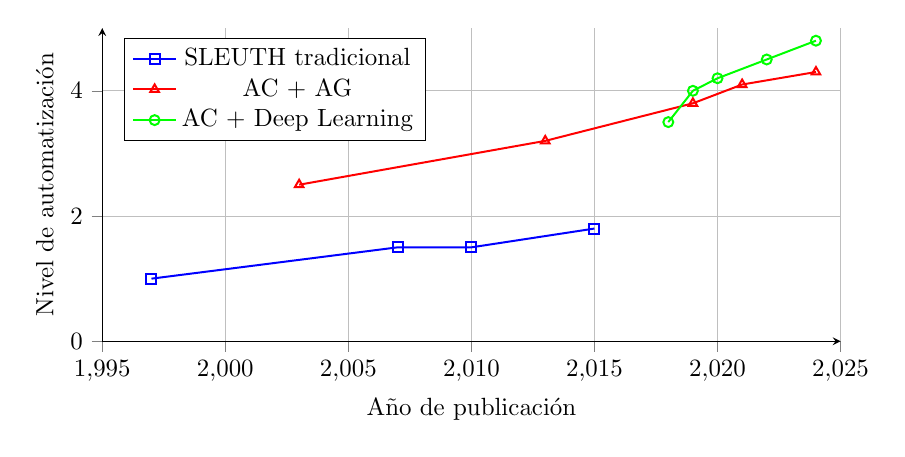
\begin{tikzpicture}[scale=0.9]
\begin{axis}[
	axis x line=bottom,
	axis y line=left,
	tick align=outside,
	every axis plot/.append style={thick},
	width=12cm,
	height=6cm,
	xlabel={Año de publicación},
	ylabel={Nivel de automatización},
	xmin=1995,
	xmax=2025,
	ymin=0,
	ymax=5,
	grid=major,
	legend pos=north west
]

% SLEUTH tradicional
\addplot[mark=square,blue,thick] coordinates {
	(1997,1) (2007,1.5) (2010,1.5) (2015,1.8)
};
\addlegendentry{SLEUTH tradicional}

% AC + GA
\addplot[mark=triangle,red,thick] coordinates {
	(2003,2.5) (2013,3.2) (2019,3.8) (2021,4.1) (2024,4.3)
};
\addlegendentry{AC + AG}

% AC + Deep Learning
\addplot[mark=o,green,thick] coordinates {
	(2018,3.5) (2019,4.0) (2020,4.2) (2022,4.5) (2024,4.8)
};
\addlegendentry{AC + Deep Learning}

\end{axis}
\end{tikzpicture}
\caption{Evolución temporal de enfoques de modelado urbano}
\label{fig:evolution_timeline}
\end{figure}

\subsection{Trabajos pioneros y fundamentales}

\subsubsection{Fundamentos teóricos}

\textbf{Wolfram (1984)} estableció las bases matemáticas de los Autómatas Celulares, demostrando cómo reglas simples pueden generar comportamientos complejos. Su trabajo proporcionó el fundamento teórico para aplicaciones posteriores en modelado espacial.

\textbf{White \& Engelen (1997)} fueron pioneros en la aplicación de AC al crecimiento urbano, desarrollando el primer modelo operativo que capturaba dinámicas de uso de suelo mediante reglas locales de transición.

\textbf{Clarke \& Gaydos (1997)} y \textbf{Clarke (2007)} desarrollaron y consolidaron el modelo SLEUTH, estableciendo el estándar de facto para modelado AC urbano durante más de dos décadas.

\subsubsection{Innovaciones en optimización evolutiva}

\textbf{Almeida et al. (2003)} realizaron el primer intento exitoso de integrar Algoritmos Genéticos con AC urbanos, demostrando la viabilidad de automatizar la calibración de parámetros y estableciendo las bases metodológicas para trabajos posteriores.

\textbf{Li \& Dang (2013)} expandieron este enfoque introduciendo optimización multi-objetivo, permitiendo el balance simultáneo de múltiples criterios de calidad del modelo. Su trabajo demostró mejoras significativas en la concordancia espacial.

\textbf{Huang et al. (2019)} integraron restricciones espaciales explícitas en el proceso de optimización, mostrando cómo incorporar conocimiento experto en el marco evolutivo sin comprometer la automatización.

\subsection{Desarrollos recientes y tendencias emergentes}

\subsubsection{Integración con inteligencia artificial}

\textbf{Wang et al. (2021)} desarrollaron enfoques híbridos que combinan AC tradicionales con redes neuronales para aprendizaje de patrones espaciales complejos, manteniendo la interpretabilidad de los AC mientras aprovechan la capacidad de aprendizaje del Deep Learning.

\textbf{Tang et al. (2024)} propusieron algoritmos evolutivos híbridos que combinan múltiples metaheurísticas, demostrando mejoras en eficiencia computacional y calidad de soluciones en problemas de calibración de AC urbanos.

\subsubsection{Avances en sensado remoto}

\textbf{Ma et al. (2019)} aplicaron redes neuronales convolucionales para detectar cambios urbanos en series temporales satelitales, logrando precisiones superiores al 95\% en clasificación binaria urbano/no-urbano.

\textbf{Kadhim et al. (2018)} desarrollaron metodologías para clasificación automática multi-clase de uso de suelo usando Deep Learning, estableciendo nuevos estándares de precisión para preparación de datos de entrada a modelos AC.

\subsection{Análisis de brechas identificadas}

\subsubsection{Limitaciones metodológicas actuales}

A pesar de los avances significativos, la literatura revela varias limitaciones persistentes:

\begin{enumerate}
	\item \textbf{Validación temporal limitada}: La mayoría de estudios utiliza solo 2-3 puntos temporales, insuficientes para validación robusta de capacidades predictivas

	\item \textbf{Falta de reproducibilidad}: Muchos trabajos no proporcionan código ni datos suficientes para replicación, limitando la verificación independiente de resultados

	\item \textbf{Integración limitada}: Pocos trabajos combinan efectivamente extracción de conocimiento espacial, optimización evolutiva y validación temporal robusta

	\item \textbf{Aplicación contextual limitada}: Escasos estudios en contextos latinoamericanos con sus particularidades específicas
\end{enumerate}

\subsubsection{Oportunidades de investigación}

Las brechas identificadas revelan oportunidades claras:

\begin{itemize}
	\item \textbf{Series temporales extensas}: Aprovechamiento de archivos satelitales históricos de 30+ años
	\item \textbf{Automatización completa}: Pipelines end-to-end desde datos crudos hasta predicciones
	\item \textbf{Validación multi-métrica}: Integración de IoU, FOM y Kappa en función objetivo única
	\item \textbf{Reproducibilidad total}: Liberación de código, datos y documentación completa
\end{itemize}

\subsection{Posicionamiento de la propuesta}

\subsubsection{Diferenciadores clave}

La presente investigación se diferencia de trabajos previos en aspectos fundamentales:

\begin{table}[b]
\centering
\caption{Diferenciadores de la propuesta vs estado del arte}
\renewcommand{\arraystretch}{1.3}
\begin{tabular}{@{}p{4cm}p{5cm}p{5cm}@{}}
\toprule
\textbf{Aspecto} & \textbf{Estado del arte} & \textbf{Esta propuesta} \\
\midrule
Extracción de conocimiento & Manual o semi-automática & WoE completamente automatizado \\
Validación temporal & 2-3 puntos temporales & 37 años (1984-2020) \\
Función objetivo & Métrica única (típicamente Kappa) & Multi-métrica (IoU + FOM + Kappa) \\
Reproducibilidad & Código parcial o no disponible & Pipeline completo open-source \\
Aplicación contextual & Principalmente países desarrollados & Contexto mexicano específico \\
Escalabilidad & Implementaciones ad-hoc & Arquitectura modular reutilizable \\
\bottomrule
\end{tabular}
\label{tab:differentiators}
\end{table}

\subsubsection{Contribuciones esperadas}

Basándose en el análisis comparativo, se esperan las siguientes contribuciones únicas:

\begin{enumerate}
	\item \textbf{Metodológica}: Primera integración completa de WoE automatizado + AG multi-objetivo + validación temporal extensa

	\item \textbf{Técnica}: Framework modular que permite extensión y adaptación a diferentes contextos urbanos

	\item \textbf{Empírica}: Validación más robusta del estado del arte usando 36 transiciones temporales

	\item \textbf{Práctica}: Herramientas directamente aplicables por instituciones mexicanas de planificación urbana
\end{enumerate}

\subsection{Síntesis comparativa}

El análisis de trabajos relacionados confirma que, aunque existen avances significativos en componentes individuales (AC, AG, análisis de imágenes satelitales), no existe en la literatura una integración completa que combine:

\begin{itemize}
	\item Extracción automática de conocimiento espacial
	\item Optimización evolutiva multi-objetivo
	\item Validación temporal robusta con series extensas
	\item Implementación completamente reproducible
	\item Aplicación en contextos latinoamericanos
\end{itemize}

Esta combinación representa una contribución significativa al campo y justifica plenamente la investigación propuesta como un avance sustantivo sobre el estado del arte actual.
